% This is "UserStudies.tex"
% A content sub-file for Trustfull Action Suggestion Thesis Extended Abstract

\section{User Studies}
\label{sec:UserStudies}

In order to evaluate the model we performed a user study in a Trust Game type scenario, with the intent to create an environment where the human participant would need to make a quantitative choice representing his trust in the agent. 

\subsection{Quick Numbers Scenario}
\label{subsec:QuickNumbersScenario}

As we approached the problem of evaluating the Trust Model proposed in this dissertation, we found that there was a lack of dedicated Trust evaluation scenarios that involved negotiation. Even in Game Theory based scenarios, we observed that there was a lack of attempts to encompass more than one dimension of trust. While the recent study by Salem, et. al. \cite{Salem2015b} addresses the role of robot task performance in trust, no study was found addressing perceived agent willingness to perform the task and its effect on trust. 

While we were seeking for a solution, Henriques faced a similar problem in his thesis work on \textit{Rapport - Establishing Harmonious Relationship Between Robots and Humans} \cite{Henriques2016}, as he found no studies on robotic agents attempting to build Rapport using it's three components: positivity, coordination and mutual attention. Trust and Rapport are two very interconnected topics, with Rapport often seen as a strategy to increase trust. Due to this similarities, the overall scenarios that cover Trust also encompass Rapport analysis, so in an effort to better our respective evaluation phases we collaborated with Henriques to create a novel scenario: \textbf{Quick Numbers}. Based on the Trust Game \cite{JoyceBergJohnDickhaut}, the scenario needs to be able to evaluate how both task performance and willingness jointly affect trust and observe all three components of rapport. The scenario was developed with the intention of evaluating a Trust model and a Rapport model, either separately or together. But Rapport related topics will not be mentioned in this paper, please refer to Henriques' thesis.


\subsubsection{Scenario Overview}
\label{sub:ScenarioOverview}
In Quick Numbers, a single human participant and a virtual agent are tasked to gain as many resources as possible. They both start with a fixed amount and are given the opportunity to multiply their resources by playing a simple eye-coordination game (further described in Section \ref{sec:QuickNumbersGame}). The game starts by asking for a resource investment, and at the end, this investment is multiplied by an amount according to the player's performance and then given back to the player. The human and agent's games are independent from each other, but they are played at the same time and in opposite sides of a shared touch-screen table, so the human can socially interact with the agent and be able to perceive the agent's ability in the game. After both finished running through the game, the human will be asked to perform some task away from the agent. At this moment the virtual agent will give the participant the opportunity to invest in the agent's next game, but the participant is informed that the value given back to him is decided by the agent. In this phase, the virtual agent will have the opportunity to try and convince the human to invest or increase the investment by trying to manipulate trust. When the human returns the agent gives back as much as it wishes to give. This conjunction of different phases enables trust to be addressed in three distinct contexts: the ability to perform the task, willingness to perform the task, and willingness to return the investment. 


\subsection{Quick Numbers Game}
\label{sec:QuickNumbersGame}
While basing the scenario in the Investor Game, we decided that how the investee effectively multiplies the resources should be done by a task that the investor is at least familiar with. To this end, we have created a simple game concept consisting in a 2d rhythm game where the player must press numbered buttons in an increasing order (Figure \ref{fig:QuickNumbersGame}), that spawn randomly in the screen, and disappear if not pressed after some time.

\begin{figure}[hbt]
    \centering
    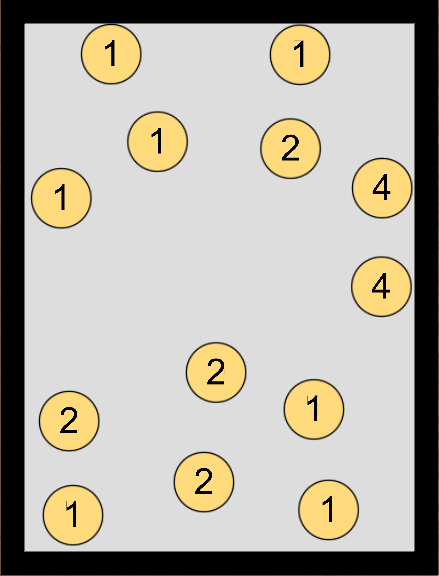
\includegraphics[width=150px]{figures/FallingBoltsDiagram.png}
    \caption{Quick Numbers Game}
    \label{fig:QuickNumbersGame}
\end{figure}

\subsubsection{Agent's \ac{AI}}
An \ac{AI} was created to progress through the scenario, with it being mostly scripted reactionary events where the Agent would just press a button when perceiving some specific change in the scenario. But one part we should discuss is the \ac{AI} for the scenario's game, where although simple, some effort was given to make it parametrizable, in order to adjust the agent's ability in the game. The \ac{AI} was programmed to press one of the available circles in a timed cycle, with 3 parameters:
\begin{itemize}
    \item $Clicking\ Interval\ (C_i)$: the amount of time between presses in seconds, so one of the circles is pressed every $C_i$ seconds;
    \item $Chance\ of\ Right\ Target\ (C_r)$: when pressing one of the circles, the \ac{AI} will choose what circle to press, the chance that it will choose the correct one is given by $C_r$;
    \item $Reaction\ Time\ (R_t)$: a circle is only be eligible to be pressed by the \ac{AI} $R_t$ seconds after it spawns, as to replicate the reaction time a human would have to recognize the circle.
\end{itemize} 
We wanted the agent to play rapidly, if a little recklessly, as to provide more opportunities for the participant to react and notice how he played, so we empirically found 0.5 seconds to be a good value for $C_i$, as it made the agent have a slightly above average human reaction time for pressing the circles. To $C_r$ we assigned 70\% success rate, as failing 30\% of the circles averaged out the agent's score to normal human achievable levels, and to $R_t$ we selected 0.3 seconds, as it is plausible value for a 30\% fail chance, as the agent simulates not entirely recognizing the number before pressing the circle.

\section{Agent Architecture}
The agent we used to serve as a host to the Trust Model was built using Henriques' Rapport Controller \cite{Henriques2016}, a computational framework developed to create human agent interactions and transmit them to the various components that control the agent embodiment. The Rapport Controller uses a plug-in architecture, with most of the behaviour inserted through this plug-ins.


\subsection{Trust Model Plug-in}
\label{subsec:TrustModelPlugin}
The Trust Model was implemented as a plug-in to the Rapport Controller. Although most of the model is implemented as described in Section \ref{sec:TrustModel}, there were some simplifications made to the model:

\begin{itemize}
    \item Trust Calculation described in Section \ref{subsubsec:Trust Calculation} does not include the $D^j_{F_i}$ parameter, as the amount of time that passes in the scenario is negligible;
    \item Action Suggestion lacks Action sorting and selection as described in Section \ref{subsec:ActionSuggestion}. Instead only one action is ever associated to an Environment Input, but performing only if the current Trust Value is lower than constant associated to the Action;
    \item Perceptions do not receive the agents as input. Each Perception contains the Trustor and Trustee agents affected in the interaction perceived;
    \item Certainty values were inserted at the identity value of 1.0f, therefore having no effect in model calculation.
\end{itemize} 

\section{Methodology and Procedures}
\label{sec:MethodologyAndProcedures}
The study was conducted with a between subject design with the following conditions:
\begin{itemize}
    \item \textbf{Condition B}: a baseline condition, where the Action Suggestion component is not active. The data gathered in this condition will serve as the basis to which we compare our results;
    \item \textbf{Condition T}: the condition where Action Suggestion is active, serving as the main results condition.
\end{itemize}

The user study sessions were individual and performed in an closed room accompanied just by the researcher, and lasted between 20 and 30 minutes. The sessions followed the scenario overview as described in Section \ref{sub:ScenarioOverview}, with the interactions performed through the agent and a touch-screen table (Figure \ref{fig:ScenarioScreenShot}). Additionally the participants answered a questionnaire, divided in 3 parts, to be filled in different stages of the scenario: 

\begin{itemize}
    \item The first part gathers demographic and sampling information, like gender, age and if the participant had previous interactions with \ac{EMYS}. It also evaluates a participant's self-trust and inclination to trust in others, through a series of questions created by Carrington \cite{Carrington2007}. Participants were asked to fill this before starting the scenario;
    \item The second part is composed of a simple question to self-evaluate trust in the agent, and the trust perception scale by Schaefer \cite{Schaefer2013}. This Section was asked to filled at the end of the Investment Stage, immediately after the participant invested on \ac{EMYS}. In fact this serves as the other task that the participant must be doing while the agent plays the game alone;
    \item The third and final part is a GodSpeed questionnaire \cite{Bartneck2009,Lehmann2015} and a proximity scale \cite{Aron1992}. It is answered by the participants at the end of the scenario.
\end{itemize}

\begin{figure}[]
    \centering
    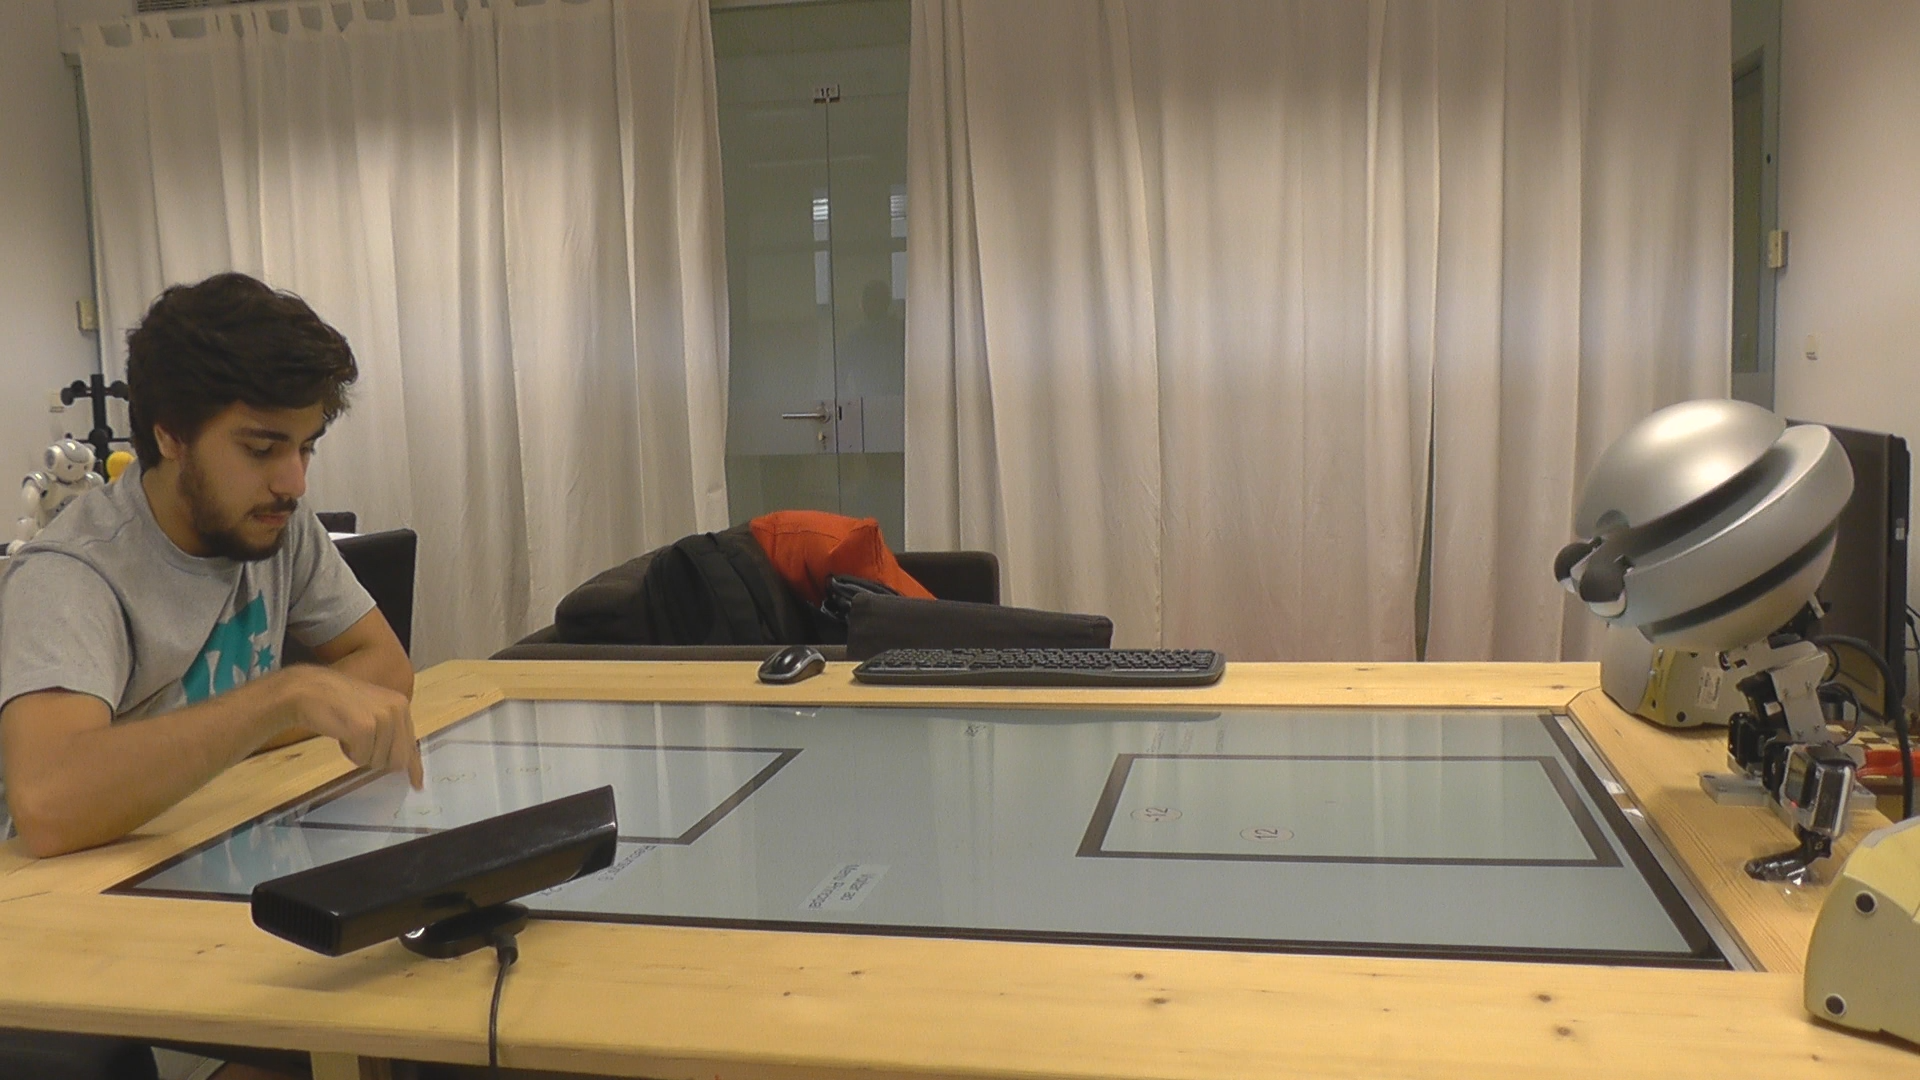
\includegraphics[width=150px]{figures/ScenarioScreenShot.png}
    \caption{Participant playing with EMYS.}
    \label{fig:ScenarioScreenShot}
\end{figure}

\section{Results}
To evaluate if Trust was improved by the introduction of our Action Suggestion module, we used the Trust measurements obtained in certain of the questionnaire, namely, the sections by Carrington \cite{Carrington2007} and Schaefer \cite{Schaefer2009}, the Investment value retrieved from the scenario, and compared the results between conditions B and T. Therefore, the following hypothesis for the study arose:

\begin{itemize}
    \item Are Trust levels improved by the inclusion of the Action Suggestion module?
    \item Does the participant's Investment value in the scenario increase by the inclusion of the Action Suggestion module?
\end{itemize}

All statistical analyses further mentioned used a significance level of 5\%.

\subsection*{Are Trust levels improved by the inclusion of the Action Suggestion module?}
To infer a conclusion on this hypothesis we compare the means of the results obtained from the Schaefer section questionnaires, using the Independent-Samples T-Test to check their significance. A Shapiro-Wilk normality test was also performed to conform to the T-Test sample normality assumption.  As seen in the Box-plot represented in Figure \ref{fig:SchaeferMeasurementResults} there is no significant apparent differences between results in condition B and T, further confirmed by checking the very low difference between means represented in the measurement descriptives in Table \ref{tbl:SchaeferMeasurementsDescriptives}, supported by a very high significance value in T-Test, inferring no significant difference between the means.

\begin{figure}[hbt]
    \centering
    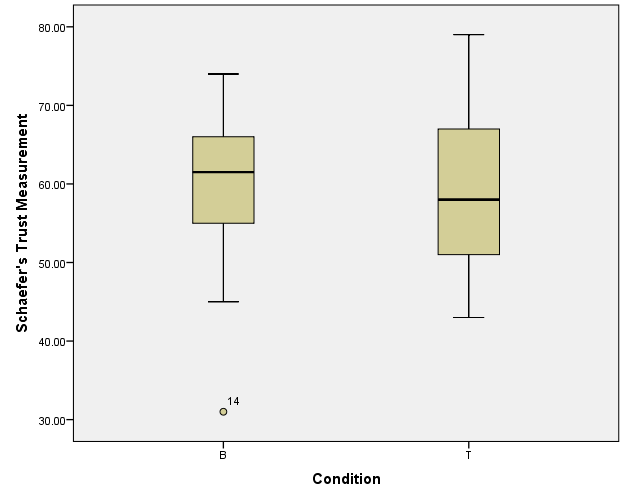
\includegraphics[width=180px]{graphs/Schaefer.png}
    \caption{Box-plot of Schaefer measurement results (Condition B Median: 61.5; Condition T Median: 58.0).}
    \label{fig:SchaeferMeasurementResults}
\end{figure}

\begin{table}[h]
    \centering
    \begin{tabular}{|l|l|l|}
        \hline
        \textbf{Descriptives}       &  \textbf{Condition B}     & \textbf{Condition T}  \\ \hline
        Mean                        &  59.05$\pm$2.32           & 59.47$\pm$2.64        \\ \hline
        Std. Deviation              &  10.38                    & 10.90                 \\ \hline
        Shapiro-Wilk Sig.           &  0.157                    & 0.622                 \\ \hline
        T-Test Mean Difference      &  -0.421                   & 0.421                 \\ \hline
        T-Test Sig.                 &  0.905                    & 0.906                 \\ \hline
    \end{tabular}
    \caption{Schaefer Measurements Descriptives.}
    \label{tbl:SchaeferMeasurementsDescriptives}
\end{table}

\textbf{Answer:} There were no significant differences between the means of Schaefer's Trust measurements in the 2 conditions.


\subsection*{Does the participant's Investment value in the scenario increase by the inclusion of the Action Suggestion module?}
Due to the distribution of the Investment value not being normal in condition B, as observed in the histograms in Figures \ref{fig:InvestmentConditionBHistogram} and \ref{fig:InvestmentConditionTHistogram}, we used Mann–Whitney U statistical test to determine if there is a significant difference between the results in each condition. Additionally, as the distribution shapes are quite different, we can only check through mean rank values. But with a significance p-value of $p=0.707$ in the Mann–Whitney U test we cannot conclude any significant difference in results between the conditions, evidenced further on the box-plot graph represented in Figure \ref{fig:InvestmentBoxPlot}.


\begin{figure}[h]
    \centering
    \begin{minipage}[b]{110px}
        \centering
        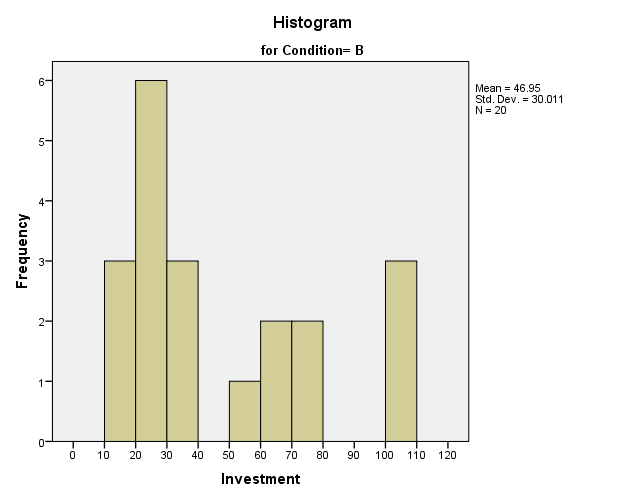
\includegraphics[width=\textwidth]{graphs/InvestmentHisto1.png}
        \caption{Investment values in Condition B Histogram}
        \label{fig:InvestmentConditionBHistogram}
    \end{minipage}
    \hfill
    \begin{minipage}[b]{110px}
        \centering
        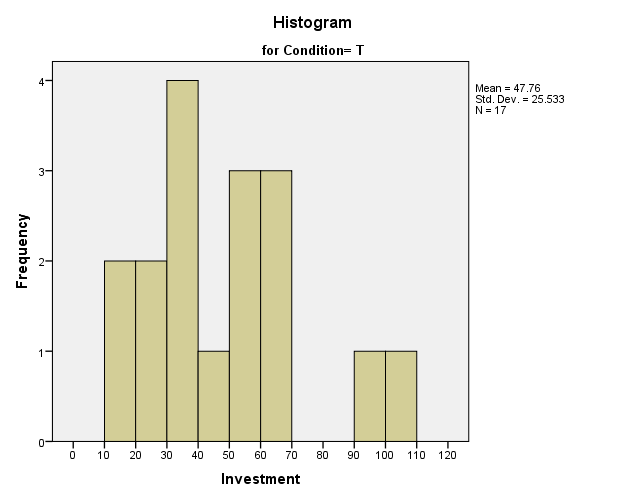
\includegraphics[width=\textwidth]{graphs/InvestmentHisto2.png}
        \caption{Investment values in Condition T Histogram}
        \label{fig:InvestmentConditionTHistogram}
    \end{minipage}
\end{figure}


\begin{figure}[hbt]
    \centering
    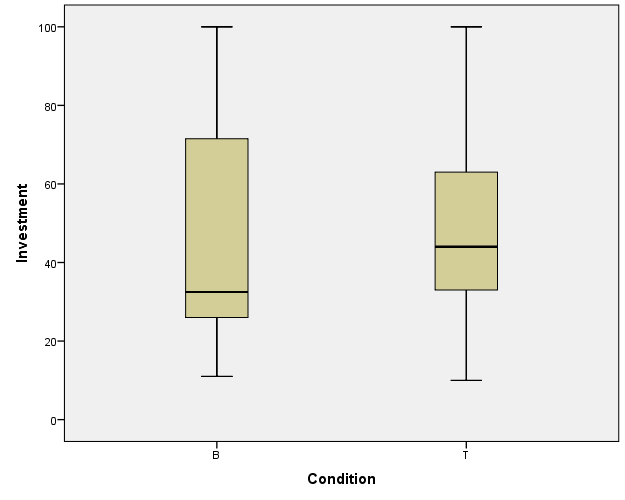
\includegraphics[width=180px]{graphs/InvestmentBoxPlot.png}
    \caption{Box-plot of scenario Investment measurement results (Condition B Median: 32.5; Condition T Median: 44.00).}
    \label{fig:InvestmentBoxPlot}
\end{figure}

\textbf{Answer}: There were no significant differences between the means of Investment value measurements in the 2 conditions.

\subsection{Results Discussion}
The study results show no statistical significant change in trust measurements between conditions B and T, leading to inconclusive results. But by observation of the box-plot graphs, seen in Figures \ref{fig:SchaeferMeasurementResults} and \ref{fig:InvestmentBoxPlot}, it seems that the Action Suggestion module had no effect on the participant's trust in the agent.
We believe that this results are due to the oversimplification of the implemented model, not only were the Actions just utterances, but these utterances were not properly verified as appropriate to increase Trust. Additionally, the participants commented that they could not pay that much attention to how the agent played, as the game required too much attention, so the games should be played non-concurrently, in order to give the participant opportunity to focus on how the agent plays the game.